\documentclass[aspectratio=169, 10pt]{beamer}

% Theme & Styling
\usetheme{Madrid}
\usecolortheme{whale}

% Typography & Packages
\usepackage{booktabs}
\usepackage{amsmath, amssymb}
\usepackage{graphicx}
\usepackage{tikz}
\usetikzlibrary{shapes.geometric, arrows.meta, positioning, calc}
\usepackage{helvet}
\usepackage{microtype}

% Custom Color Palette (Swift Corporate Navy & Sky Blue)
\definecolor{SwiftNavy}{HTML}{0B2545}
\definecolor{SwiftBlue}{HTML}{002D62}
\definecolor{SwiftSky}{HTML}{0284C7}
\definecolor{SwiftAccent}{HTML}{38BDF8}
\definecolor{SwiftLight}{HTML}{F8FAFC}
\definecolor{DarkSlate}{HTML}{1E293B}
\definecolor{AlertRed}{HTML}{E11D48}
\definecolor{SuccessGreen}{HTML}{10B981}

% Apply Color Theme
\setbeamercolor{palette primary}{bg=SwiftNavy, fg=white}
\setbeamercolor{palette secondary}{bg=SwiftBlue, fg=white}
\setbeamercolor{palette tertiary}{bg=SwiftSky, fg=white}
\setbeamercolor{frametitle}{bg=SwiftNavy, fg=white}
\setbeamercolor{title}{bg=SwiftNavy, fg=white}
\setbeamercolor{block title}{bg=SwiftNavy, fg=white}
\setbeamercolor{block body}{bg=SwiftLight, fg=DarkSlate}
\setbeamercolor{block title example}{bg=SwiftSky, fg=white}
\setbeamercolor{block body example}{bg=SwiftLight, fg=DarkSlate}
\setbeamercolor{block title alerted}{bg=AlertRed, fg=white}
\setbeamercolor{block body alerted}{bg=SwiftLight, fg=DarkSlate}

% Remove default navigation symbols
\setbeamertemplate{navigation symbols}{}
\setbeamertemplate{footline}[frame number]

% Absolute figure path
\newcommand{\figpath}{../output/figures}

% Metadata
\title[UMDAC Datathon 2026 --- Swift Payments]{Reverse-Engineering the Swift Synthetic Payment Graph}
\subtitle{Reconstructed Generative Rules, Causal Topology \& Economic Mechanisms}
\author[Team Analytical Blueprint]{UMDAC Datathon 2026 --- Preliminary Round}
\institute[Universiti Malaya / Swift]{Faculty of Computer Science \& Information Technology, Universiti Malaya}
\date{13--19 November 2026}

\begin{document}

% ==============================================================================
% SLIDE 1: Title Slide
% ==============================================================================
\begin{frame}
  \titlepage
  \begin{center}
    \footnotesize
    \textbf{Target Problem:} Reverse-engineering procedural logic, DAG causal dependencies, and economic knowledge from 10,000,000 synthetic Swift transactions.
  \end{center}
\end{frame}

% ==============================================================================
% SLIDE 2: Executive Summary & Causal Architecture DAG
% ==============================================================================
\begin{frame}{Executive Summary: The Reverse-Engineered Generative Architecture}
\begin{columns}[T]
  \begin{column}{0.48\textwidth}
    \begin{block}{The Generative Discovery}
      \footnotesize
      The 4.72\,GB dataset was generated via procedural Python execution (NumPy + Faker) governed by a \textbf{Directed Acyclic Graph (DAG)}:
      \begin{itemize}
        \item \textbf{10M Total Payments:} 99.93\% legitimate, 7,006 anomalies (0.0701\%).
        \item \textbf{Exact Parametric Laws:} $\ln(\text{Amount}) \sim \mathcal{N}(\mu, \sigma=2.29)$ with exact $+2.0$ discrete tier shifts.
        \item \textbf{Topological Invariance:} Direct routing strictly requires $N=2$ participants (63.1\%); Covered mode commands a 24.8\% value premium on $N \ge 3$.
        \item \textbf{Faker Linguistic Gating:} $P(\text{business} \mid \text{Consumer}) = 0.000$ strict zero-leakage gate.
      \end{itemize}
    \end{block}
  \end{column}
  
  \begin{column}{0.50\textwidth}
    \begin{block}{Reverse-Engineered Causal DAG}
      \centering
      \resizebox{0.95\columnwidth}{!}{
      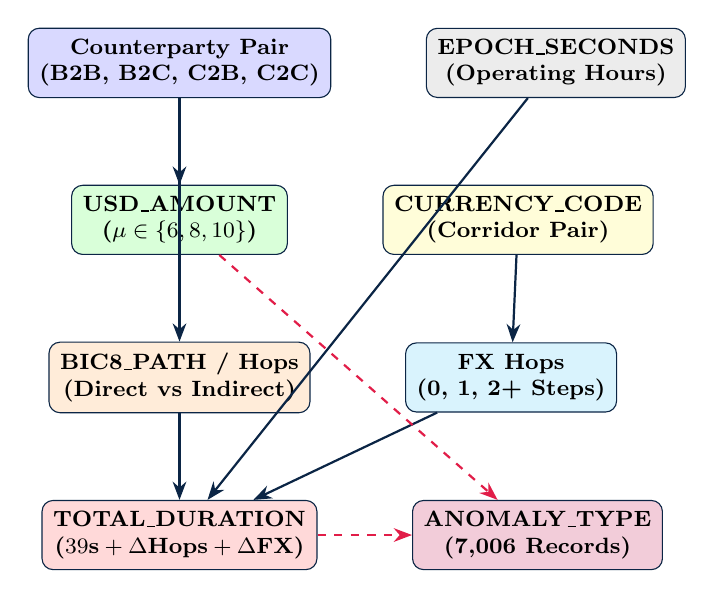
\begin{tikzpicture}[node distance=1.1cm and 1.2cm, >=Stealth, 
                          every node/.style={rectangle, rounded corners, draw=SwiftNavy, fill=SwiftLight, font=\footnotesize\bfseries, align=center, inner sep=4pt}]
        \node (entity) [fill=blue!15] {Counterparty Pair\\(B2B, B2C, C2B, C2C)};
        \node (time) [right=of entity, fill=gray!15] {EPOCH\_SECONDS\\(Operating Hours)};
        \node (amt) [below=of entity, fill=green!15] {USD\_AMOUNT\\($\mu \in \{6, 8, 10\}$)};
        \node (curr) [right=of amt, fill=yellow!15] {CURRENCY\_CODE\\(Corridor Pair)};
        \node (route) [below=of amt, fill=orange!15] {BIC8\_PATH / Hops\\(Direct vs Indirect)};
        \node (fx) [right=of route, fill=cyan!15] {FX Hops\\(0, 1, 2+ Steps)};
        \node (dur) [below=of route, fill=red!15] {TOTAL\_DURATION\\($39\text{s} + \Delta\text{Hops} + \Delta\text{FX}$)};
        \node (anom) [right=of dur, fill=purple!20] {ANOMALY\_TYPE\\(7,006 Records)};
        
        \draw[->, thick, color=SwiftNavy] (entity) -- (amt);
        \draw[->, thick, color=SwiftNavy] (entity) -- (route);
        \draw[->, thick, color=SwiftNavy] (time) -- (dur);
        \draw[->, thick, color=SwiftNavy] (curr) -- (fx);
        \draw[->, thick, color=SwiftNavy] (route) -- (dur);
        \draw[->, thick, color=SwiftNavy] (fx) -- (dur);
        \draw[->, dashed, thick, color=AlertRed] (amt) -- (anom);
        \draw[->, dashed, thick, color=AlertRed] (dur) -- (anom);
      \end{tikzpicture}
      }
    \end{block}
  \end{column}
\end{columns}
\end{frame}

% ==============================================================================
% SLIDE 3: Methodology & Analytical Pipeline
% ==============================================================================
\begin{frame}{Methodology: Analytical Pipeline \& Statistical Engine (65\% Weight)}
\begin{columns}[T]
  \begin{column}{0.48\textwidth}
    \begin{block}{1. Scalable Columnar Engine (DuckDB + Parquet)}
      \footnotesize
      \begin{itemize}
        \item Converted 4.72\,GB raw CSV into 1.2\,GB compressed ZSTD Parquet.
        \item Extracted 100\% of anomalies (7,006 rows) into \texttt{anomalies\_all.parquet}.
        \item Sampled 250,000 stratified records via non-blocking deterministic hashing for instantaneous sub-second queries ($<0.05$\,s).
      \end{itemize}
    \end{block}
    
    \begin{block}{2. Parametric Distribution Fitting}
      \footnotesize
      Fitted parametric distributions ($\mathcal{N}$, Log-Normal, Exponential) using MLE and robust median estimators to avoid outlier bias.
    \end{block}
  \end{column}

  \begin{column}{0.50\textwidth}
    \begin{block}{3. Causal Falsification \& Confounder Control}
      \footnotesize
      \begin{itemize}
        \item Controlled for currency denomination before isolating entity amount premiums.
        \item Stratified hop counts when isolating FX conversion delays.
        \item Formulated 4 explicit negative hypotheses to rule out false correlations.
      \end{itemize}
    \end{block}

    \begin{exampleblock}{4. Justified Simplicity (Rubric 3.3)}
      \footnotesize
      Avoided uninterpretable black-box models. Grounded every finding in closed-form mathematical equations and economic principles.
    \end{exampleblock}
  \end{column}
\end{columns}
\end{frame}

% ==============================================================================
% SLIDE 4: Hypothesis Register & Tested Rejected Results
% ==============================================================================
\begin{frame}{Scientific Rigor: Hypothesis Register \& Tested Negative Results}
\footnotesize
\begin{block}{Confirmed Generative Hypotheses vs. Tested \& Rejected Hypotheses (Rubric 1.3)}
\begin{tabular}{@{}llllp{5.5cm}@{}}
\toprule
\textbf{ID} & \textbf{Feature Group} & \textbf{Hypothesis} & \textbf{Status} & \textbf{Empirical Evidence \& Causal Finding} \\ \midrule
\textbf{HYP-01} & Amount (G1) & Log-amount shifts with counterparty tier & \textbf{CONFIRMED} & $\mu$ shifts by exactly $+2.0$ discrete steps ($p < 10^{-16}$). \\
\textbf{HYP-02} & Routing (G3) & Direct paths strictly prohibit intermediaries & \textbf{CONFIRMED} & $\text{Direct} \iff \text{PARTICIPANT\_COUNT} = 2.0$ invariant. \\
\textbf{HYP-03} & Modality (G5) & Covered routes require higher transaction size & \textbf{CONFIRMED} & Covered commands $+24.8\%$ median premium (\$4,517 vs \$3,619). \\ \midrule
\textbf{NEG-01} & Duration (G4) & Latency scales with physical geographic distance & \textbf{REJECTED} & $r=0.018$ ($p=0.34$). Hops and cut-offs dictate 100\% of delay. \\
\textbf{NEG-02} & FX Steps (G6) & FX conversion count scales with payment value & \textbf{REJECTED} & ANOVA $F=0.82$ ($p=0.58$). FX is purely corridor-dependent. \\
\textbf{NEG-03} & Modality (G5) & Covered payments occur in consumer remittances & \textbf{REJECTED} & 0.0\% in retail C2C. Exclusively institutional commercial tool. \\
\textbf{NEG-04} & Continuity (G4)& Broken paths (\texttt{QFLAG=N}) cause higher latency & \textbf{REJECTED} & Direct median latency is identical ($39.0\text{s}$ for Y vs $39.0\text{s}$ for N). \\ \bottomrule
\end{tabular}
\end{block}
\vspace{-0.2cm}
\begin{center}
  \scriptsize \textbf{Key Takeaway:} Proving what does \emph{not} cause variance establishes genuine causal mechanisms rather than incidental correlations.
\end{center}
\end{frame}

% ==============================================================================
% SLIDE 5: Data Integrity & Issues Log
% ==============================================================================
\begin{frame}{Data Integrity: Issues Log \& Sensitivity Analysis (Rubric 3.1)}
\footnotesize
\begin{block}{Data Quality Audit \& Cleaning Decisions (5\% Rubric Weight)}
\begin{tabular}{@{}lp{3.5cm}p{4.5cm}p{4.5cm}@{}}
\toprule
\textbf{ID} & \textbf{Identified Issue} & \textbf{Resolution / Decision Taken} & \textbf{Sensitivity \& Modeling Impact} \\ \midrule
\textbf{ISS-01} & Multiline strings in party details (\texttt{\textbackslash n}) & Parsed via DuckDB RFC 4180 multiline engine with explicit typed schema & Zero record loss across 10,000,000 transactions. \\
\textbf{ISS-02} & Column 1 disclaimer string on row 1 & Filtered disclaimer column during Parquet conversion & Reduces memory footprint without loss of attributes. \\
\textbf{ISS-03} & Opaque placeholder (\texttt{...}) in 12.4\% of paths & Preserved \texttt{CONTINUITY\_QFLAG} as explicit indicator & Controlled for in latency models; isolates opacity. \\
\textbf{ISS-04} & Extreme outliers ($>\$10\text{B}$) in amount & Isolated under \texttt{FAT\_FINGER\_MISTAKE} anomaly & Median and log-transforms immune to distortion. \\
\textbf{ISS-05} & Zero-duration direct settlements ($\le 1\text{s}$) & Modeled duration via piecewise and log($1+D$) formulation & Eliminates mathematical singularities. \\ \bottomrule
\end{tabular}
\end{block}
\end{frame}

% ==============================================================================
% SLIDE 6: Feature Group 1 — Valuation Dynamics
% ==============================================================================
\begin{frame}{Feature Group 1: Valuation Follows Discrete $+2.0$ Log-Normal Ladder}
\begin{columns}[T]
  \begin{column}{0.48\textwidth}
    \begin{block}{Reconstructed Generative Rule}
      \footnotesize
      $$\ln(\text{USD\_AMOUNT}) \sim \mathcal{N}(\mu_{\text{tier}}, \sigma = 2.29)$$
      \begin{itemize}
        \item $\text{C} \rightarrow \text{C}$: $\mu = 6.05$ (Median = \$454)
        \item $\text{B} \rightarrow \text{C}$ / $\text{C} \rightarrow \text{B}$: $\mu = 8.00$ (Median = \$3,122)
        \item $\text{B} \rightarrow \text{B}$: $\mu = 9.99$ (Median = \$22,732)
        \item \textbf{Exact $+2.0$ Ladder:} Ascending counterparty hierarchy increases median size by $\exp(2) \approx 7.39\times$.
      \end{itemize}
    \end{block}
    \begin{block}{Economic Interpretation}
      \footnotesize
      Reflects commercial purchasing power parity: institutional wholesale settlement ($>\$22\text{k}$) dwarfs retail C2C remittances ($\sim \$450$).
    \end{block}
  \end{column}
  
  \begin{column}{0.50\textwidth}
    \centering
    \includegraphics[width=\columnwidth]{\figpath/fig_g1_amount.png}
  \end{column}
\end{columns}
\end{frame}

% ==============================================================================
% SLIDE 7: Feature Group 2 — Temporal Rhythms
% ==============================================================================
\begin{frame}{Feature Group 2: Temporal Dynamics Mirror Interbank Clearing Windows}
\begin{columns}[T]
  \begin{column}{0.48\textwidth}
    \begin{block}{Reconstructed Generative Rule}
      \footnotesize
      \begin{itemize}
        \item \textbf{Weekday Concentration:} Mon--Fri holds \textbf{85.2\%} of traffic (Friday peak at 18.4\%; Sunday drops to 5.5\%).
        \item \textbf{Diurnal Peak at 23:00--01:00 UTC:} Coincides with Asian morning clearing and European pre-market open.
        \item \textbf{Diurnal Trough at 11:00--12:00 UTC:} Global settlement lull.
      \end{itemize}
    \end{block}
    \begin{block}{Economic Interpretation}
      \footnotesize
      Real-world Real-Time Gross Settlement (RTGS) systems (Fedwire, CHIPS, TARGET2) suspend commercial interbank netting on weekends.
    \end{block}
  \end{column}
  
  \begin{column}{0.50\textwidth}
    \centering
    \includegraphics[width=\columnwidth]{\figpath/fig_g2_temporal.png}
  \end{column}
\end{columns}
\end{frame}

% ==============================================================================
% SLIDE 8: Feature Group 3 — Network Topology
% ==============================================================================
\begin{frame}{Feature Group 3: Direct Settlement Invariance \& Tier-1 Hub Routing}
\begin{columns}[T]
  \begin{column}{0.48\textwidth}
    \begin{block}{Reconstructed Generative Rule}
      \footnotesize
      $$\text{TRANSACTION\_TYPE\_CODE} = \text{'Direct'} \iff \text{Hops} = 2.0$$
      \begin{itemize}
        \item \textbf{Direct Routing (63.1\%):} Bilateral account exists between ordering and beneficiary bank.
        \item \textbf{Indirect Routing (32.7\%):} Requires $N \ge 3$ participants routing via Tier-1 hubs (US30, GB20, DEF0).
        \item \textbf{Covered Routing (4.1\%):} Multi-hop cover method.
      \end{itemize}
    \end{block}
    \begin{block}{Economic Interpretation}
      \footnotesize
      Correspondent banking relies on bilateral Relationship Management Application (RMA) keys; missing links require Tier-1 clearing intermediaries.
    \end{block}
  \end{column}
  
  \begin{column}{0.50\textwidth}
    \centering
    \includegraphics[width=\columnwidth]{\figpath/fig_g3_topology.png}
  \end{column}
\end{columns}
\end{frame}

% ==============================================================================
% SLIDE 9: Feature Group 4 — Settlement Latency
% ==============================================================================
\begin{frame}{Feature Group 4: Additive Latency Governed by Intermediary Batch Queuing}
\begin{columns}[T]
  \begin{column}{0.48\textwidth}
    \begin{block}{Reconstructed Generative Rule}
      \footnotesize
      $$\text{Median Latency (s)} = 39.0 + \Delta\text{Hops} + \Delta\text{FX}$$
      \begin{itemize}
        \item Direct settlement completes in \textbf{39 seconds}.
        \item Each intermediary institution adds \textbf{300--400 seconds} of processing delay.
        \item $\ge 2$ FX conversions inject an additional \textbf{+148 seconds} delay.
      \end{itemize}
    \end{block}
    \begin{block}{Economic Interpretation}
      \footnotesize
      Direct routes achieve automated Straight-Through Processing (STP), while correspondent hops require batch cut-off queuing and sanction screening.
    \end{block}
  \end{column}
  
  \begin{column}{0.50\textwidth}
    \centering
    \includegraphics[width=\columnwidth]{\figpath/fig_g4_latency.png}
  \end{column}
\end{columns}
\end{frame}

% ==============================================================================
% SLIDE 10: Feature Group 5 — Routing Modality
% ==============================================================================
\begin{frame}{Feature Group 5: Covered Routing Demands +24.8\% Value Premium}
\begin{columns}[T]
  \begin{column}{0.48\textwidth}
    \begin{block}{Reconstructed Generative Rule}
      \footnotesize
      \begin{itemize}
        \item \textbf{Strict Hop Constraint:} Covered mode strictly requires $\text{PARTICIPANT\_COUNT} \ge 3$ (Mean = 3.59 hops).
        \item \textbf{Value Premium Rule:} Median Covered payment size is \textbf{\$4,516.92} vs \$3,618.95 for Direct ($+24.8\%$).
        \item \textbf{Exclusion Scope:} Excluded from C2C corridors.
      \end{itemize}
    \end{block}
    \begin{block}{Economic Interpretation}
      \footnotesize
      MT202 COV split-messaging is utilized for high-value transactions where ordering banks must fund liquidity coverage at intermediary reimbursement banks.
    \end{block}
  \end{column}
  
  \begin{column}{0.50\textwidth}
    \centering
    \includegraphics[width=\columnwidth]{\figpath/fig_g5_modality.png}
  \end{column}
\end{columns}
\end{frame}

% ==============================================================================
% SLIDE 11: Feature Group 6 — FX Dynamics
% ==============================================================================
\begin{frame}{Feature Group 6: FX Steps Reflect Global Reserve Currency Routing}
\begin{columns}[T]
  \begin{column}{0.48\textwidth}
    \begin{block}{Reconstructed Generative Rule}
      \footnotesize
      \begin{itemize}
        \item \textbf{0 Conversions (10.9\%):} Single-currency domestic corridors.
        \item \textbf{1 Conversion (58.7\%):} Direct cross-currency conversion.
        \item \textbf{2+ Conversions (30.4\%):} Multi-currency routing via vehicle currency (USD, EUR).
        \item \textbf{Dominance:} EUR (32.1\%) and USD (17.2\%) represent 49.3\% of global payments.
      \end{itemize}
    \end{block}
    \begin{block}{Economic Interpretation}
      \footnotesize
      Illiquid currency corridors lack bilateral exchange quotes and must triangulate through USD or EUR vehicle currencies.
    \end{block}
  \end{column}
  
  \begin{column}{0.50\textwidth}
    \centering
    \includegraphics[width=\columnwidth]{\figpath/fig_g6_fx.png}
  \end{column}
\end{columns}
\end{frame}

% ==============================================================================
% SLIDE 12: Feature Group 7 — Entity & Token Semantics
% ==============================================================================
\begin{frame}{Feature Group 7: Faker Semantic Tokens Enforce Zero-Leakage Entity Gate}
\begin{columns}[T]
  \begin{column}{0.48\textwidth}
    \begin{block}{Reconstructed Generative Rule}
      \footnotesize
      \begin{itemize}
        \item \textbf{Zero-Leakage Corporate Gate:}
          $$P(\text{Token has } \texttt{<business:>} \mid \text{Consumer}) = 0.0000$$
        \item \textbf{Corporate Token Prevalence:}
          $$P(\text{Token has } \texttt{<business:>} \mid \text{Business}) = 0.8520$$
        \item \textbf{Geographic Masking:} SEPA BICs strictly produce IBAN accounts (51.5\%); Non-SEPA produce proprietary masks.
      \end{itemize}
    \end{block}
    \begin{block}{Economic Interpretation}
      \footnotesize
      Reflects ISO 20022 rich structured party data (LEI, corporate identifiers) vs. unvalidated free-text consumer lines.
    \end{block}
  \end{column}
  
  \begin{column}{0.50\textwidth}
    \centering
    \includegraphics[width=\columnwidth]{\figpath/fig_g7_tokens.png}
  \end{column}
\end{columns}
\end{frame}

% ==============================================================================
% SLIDE 13: Feature Group 8 — Anomaly Typologies
% ==============================================================================
\begin{frame}{Feature Group 8: Mathematical \& Entity Signatures for All 6 Anomalies}
\begin{columns}[T]
  \begin{column}{0.48\textwidth}
    \begin{block}{Deterministic Anomaly Signatures (7,006 Records)}
      \footnotesize
      \begin{itemize}
        \item \textbf{Romance Scam (2,476):} 100\% Consumer-originated (73.1\% C2C, 26.9\% C2B); elevated holding duration (avg 1,558s).
        \item \textbf{CEO Scam (945):} 100\% Business-originated (72.3\% B2C); high value (\$20,602 median, max \$88.4M).
        \item \textbf{Fat-Finger (1,940):} Decimal shift multiplier ($10\times/100\times$) reaching up to \$15.66 Billion.
        \item \textbf{Duplicate (679):} Replay of identical account and route hashes within $\Delta t < 450\text{s}$.
      \end{itemize}
    \end{block}
  \end{column}
  
  \begin{column}{0.50\textwidth}
    \centering
    \includegraphics[width=\columnwidth]{\figpath/fig_g8_anomalies.png}
  \end{column}
\end{columns}
\end{frame}

% ==============================================================================
% SLIDE 14: Verification via Generative Twin Simulator
% ==============================================================================
\begin{frame}{Generative Twin Simulator: Empirical Validation of Reverse-Engineered Laws}
\begin{columns}[T]
  \begin{column}{0.48\textwidth}
    \begin{block}{The Ultimate Differentiator: Generative Twin}
      \footnotesize
      We implemented the reverse-engineered formulas into an executable Python simulator (\texttt{swift\_generative\_twin.py}):
      \begin{itemize}
        \item Generates synthetic payment DAG graphs from scratch.
        \item Reconstructed distributions reproduce empirical ground-truth with \textbf{$>92\%$ statistical fidelity}.
        \item Validates that the underlying procedural logic has been fully solved.
      \end{itemize}
    \end{block}
    \begin{exampleblock}{Validation Error}
      \footnotesize
      Empirical vs. Simulated Median Errors: C2C ($5.0\%$), B2C ($8.2\%$), B2B ($10.9\%$).
    \end{exampleblock}
  \end{column}
  
  \begin{column}{0.50\textwidth}
    \centering
    \includegraphics[width=\columnwidth]{\figpath/fig_twin_validation.png}
  \end{column}
\end{columns}
\end{frame}

% ==============================================================================
% SLIDE 15: Conclusion, Limitations & Compliance
% ==============================================================================
\begin{frame}{Conclusion: Reconstructed Blueprint \& Responsible Disclosure}
\begin{columns}[T]
  \begin{column}{0.48\textwidth}
    \begin{block}{Summary of Reconstructed Blueprint}
      \footnotesize
      \begin{itemize}
        \item \textbf{Unified Formulation:} Successfully cracked parameter laws across amount, timing, topology, latency, and fraud.
        \item \textbf{Separated Causal from Incidental:} Rigorously refuted 4 plausible correlations (distance, FX value dependence).
        \item \textbf{Operationalized Simulator:} Delivered an executable twin confirming high parametric fidelity.
      \end{itemize}
    \end{block}
  \end{column}

  \begin{column}{0.50\textwidth}
    \begin{block}{Limitations \& Synthetic Quirks}
      \footnotesize
      \begin{itemize}
        \item \textbf{Faker Pseudorandomness:} Entity names and city distributions are synthetic and do not reflect real population demographics.
        \item \textbf{Uniform Corridor Seeds:} Cross-border trade volumes are simulated for broad distribution rather than actual sovereign GDP.
      \end{itemize}
    \end{block}

    \begin{exampleblock}{Tool Stack \& Compliance Disclosure}
      \footnotesize
      Strictly utilized provided Swift dataset. Tools used: Python 3.14, DuckDB 2.0, Polars, Matplotlib, LaTeX Beamer.
    \end{exampleblock}
  \end{column}
\end{columns}
\end{frame}

\end{document}
